\documentclass[t,usenames,dvipsnames]{beamer}
\usetheme{Copenhagen}
\setbeamertemplate{headline}{} % remove toc from headers
\beamertemplatenavigationsymbolsempty

\usepackage{amsmath, xcolor, tikz, pgfplots}

\pgfplotsset{compat = 1.16}
\usetikzlibrary{arrows.meta, calc, decorations.pathreplacing}
\pgfplotsset{every axis/.append style = {axis lines = middle}}
\pgfplotsset{every tick label/.append style={font=\scriptsize}}
\everymath{\displaystyle}

\title{Quadratic Functions}
\author{}
\date{}

\AtBeginSection[]
{
  \begin{frame}
    \frametitle{Objectives}
    \tableofcontents[currentsection]
  \end{frame}
}

\begin{document}

\begin{frame}
    \maketitle
\end{frame}

\section{Determine the vertex, range, and intercepts of a quadratic function in standard form}

\begin{frame}{Quadratic Functions}
A \alert{quadratic function} is a function in the form
\[ f(x) = ax^2 + bx + c \]
where $a$, $b$, and $c$ are real numbers with $a \neq 0$.   \newline\\

The domain of a quadratic function is $(-\infty, \infty)$.
\end{frame}

\begin{frame}{Graph of a Quadratic Function}
For $f(x) = x^2$, the graph below is a \alert{parabola}.
\begin{center}
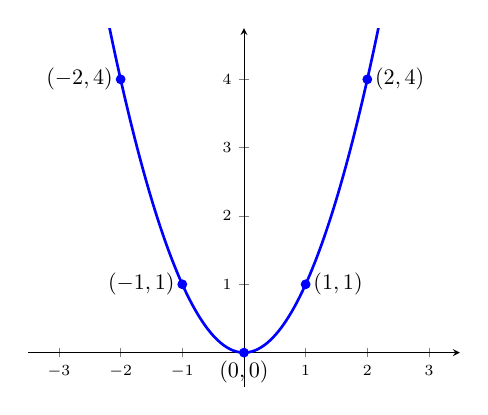
\begin{tikzpicture}[scale=0.8]
\begin{axis}[
xmin = -3.5, xmax = 3.5,
ymin = -0.5, ymax = 4.75,
xtick = {-3,-2,...,3},
ytick = {1,2,3,4}
]
\addplot[color=blue, very thick, samples=200, smooth] {x^2};
\addplot[color=blue, mark=*, only marks] coordinates {(-2,4) (-1,1) (0,0) (1,1) (2,4)};
\node at (axis cs:-2,4) [left] {$(-2,4)$};
\node at (axis cs:-1,1) [left] {$(-1,1)$};
\node at (axis cs:0,0) [below] {$(0,0)$};
\node at (axis cs:1,1) [right] {$(1,1)$};
\node at (axis cs:2,4) [right] {$(2,4)$};
\end{axis}
\end{tikzpicture}
\end{center}
\end{frame}

\begin{frame}{Graph of a Quadratic Function}
The point $(0,0)$ is called the \alert{vertex} of the parabola and can be either a relative minimum or relative maximum point. \newline\\  \pause

We can graph parabolas using transformations to the parent function $f(x) = x^2$.
\end{frame}

\begin{frame}{Example 1}
Graph the following functions starting with the graph of $f(x) = x^2$ and using transformations. Find the vertex, state the range, and find the $x$- and $y$-intercepts, if any exist.   \newline\\
(a) \quad $g(x) = (x+2)^2 - 3$  \newline\\
\begin{minipage}{0.55\textwidth}
\onslide<2->{
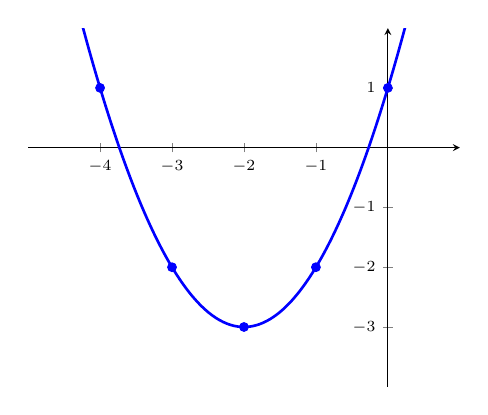
\begin{tikzpicture}[scale=0.8]
\begin{axis}[
xmin = -5, xmax = 1,
ymin = -4, ymax = 2,
xtick = {-4,-3,-2,-1,0},
ytick = {-3,-2,-1,0,1}
]
\addplot[color=blue, very thick, samples=200, smooth] {(x+2)^2 - 3};
\addplot[color=blue, mark=*, only marks] coordinates {(-4,1) (-3,-2) (-2,-3) (-1,-2) (0,1)};
\end{axis}
\end{tikzpicture}}
\end{minipage}
\begin{minipage}{0.4\textwidth}
\onslide<3->{
Shift left 2 units \\\\
Shift down 3 units }
\end{minipage}
\end{frame}

\begin{frame}{Example 1}
(a) \quad $g(x) = (x+2)^2 - 3$  \newline\\
\begin{minipage}{0.55\textwidth}
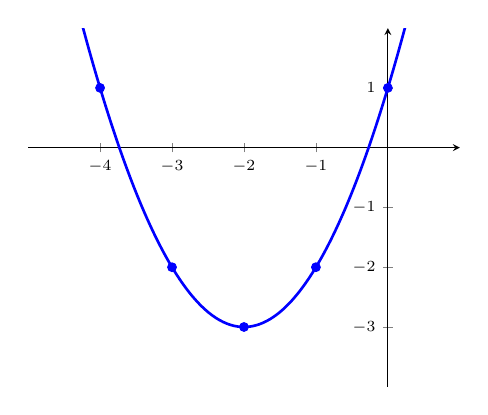
\begin{tikzpicture}[scale=0.8]
\begin{axis}[
xmin = -5, xmax = 1,
ymin = -4, ymax = 2,
xtick = {-4,-3,-2,-1,0},
ytick = {-3,-2,-1,0,1}
]
\addplot[color=blue, very thick, samples=200, smooth] {(x+2)^2 - 3};
\addplot[color=blue, mark=*, only marks] coordinates {(-4,1) (-3,-2) (-2,-3) (-1,-2) (0,1)};
\end{axis}
\end{tikzpicture}
\end{minipage}
\begin{minipage}{0.4\textwidth}
\onslide<2->{Vertex at $(-2,-3)$} \\[8pt]
\onslide<3->{Range $[-3, \infty)$} \\[8pt]
\onslide<4->{$x$-intercepts:} 
\begin{align*}
\onslide<4->{(x+2)^2 - 3 &= 0} \\
\onslide<5->{(x+2)^2 &= 3} \\
\onslide<6->{x+2 &= \pm \sqrt{3}} \\
\onslide<7->{x &= -2\pm \sqrt{3}}
\end{align*}
\onslide<8->{$(-2\pm \sqrt{3}, 0)$}
\end{minipage}
\end{frame}

\begin{frame}{Example 1}
(a) \quad $g(x) = (x+2)^2 - 3$  \newline\\
\begin{minipage}{0.55\textwidth}
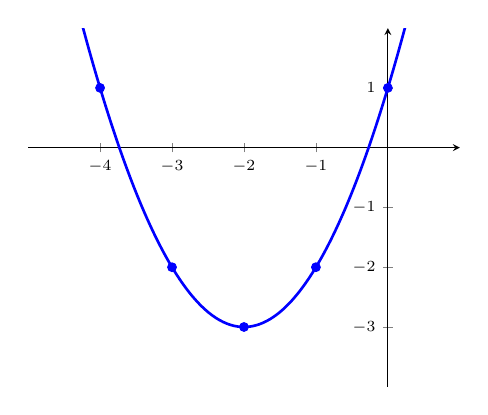
\begin{tikzpicture}[scale=0.8]
\begin{axis}[
xmin = -5, xmax = 1,
ymin = -4, ymax = 2,
xtick = {-4,-3,-2,-1,0},
ytick = {-3,-2,-1,0,1}
]
\addplot[color=blue, very thick, samples=200, smooth] {(x+2)^2 - 3};
\addplot[color=blue, mark=*, only marks] coordinates {(-4,1) (-3,-2) (-2,-3) (-1,-2) (0,1)};
\end{axis}
\end{tikzpicture}
\end{minipage}
\begin{minipage}{0.4\textwidth}
\onslide<2->{$y$-intercept at $(0,1)$}
\end{minipage}
\end{frame}

\begin{frame}{Example 1}
(b) \quad $h(x) = -2(x-3)^2 + 1$    \newline\\
\begin{minipage}{0.55\textwidth}
\onslide<2->{
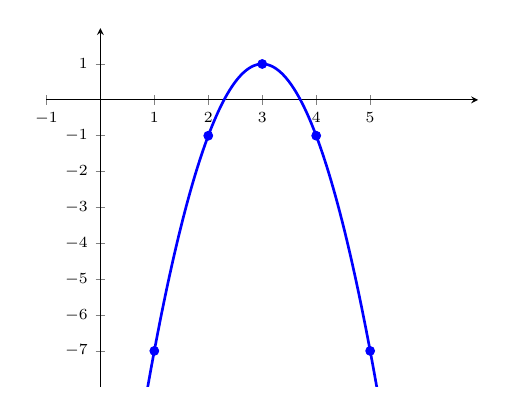
\begin{tikzpicture}[scale=0.8]
\begin{axis}[
xmin = -1, xmax = 7,
ymin = -8, ymax = 2,
xtick = {-1,0,...,5},
ytick = {-7,-6,...,1}
]
\addplot[color=blue, very thick, samples=200, smooth, domain=0:6] {-2*(x-3)^2 + 1};
\addplot[color=blue, mark=*, only marks] coordinates {(1,-7) (2,-1) (3,1) (4,-1) (5,-7)};
\end{axis}
\end{tikzpicture}}
\end{minipage}
\begin{minipage}{0.4\textwidth}
\onslide<3->{
Reflect across $x$-axis \\\\
Vertical stretch by factor of 2 \\\\
Shift right 3 units \\\\
Shift up 1 unit}
\end{minipage}
\end{frame}

\begin{frame}{Example 1}
(b) \quad $h(x) = -2(x-3)^2 + 1$    \newline\\
\begin{minipage}{0.55\textwidth}
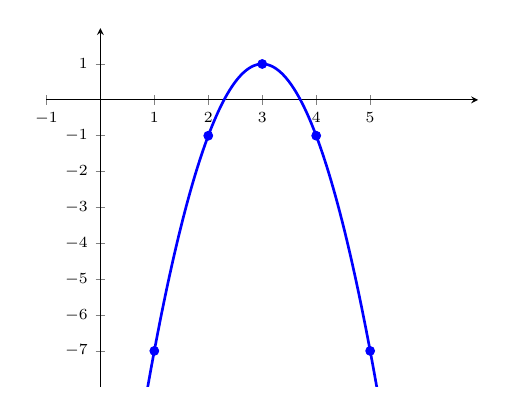
\begin{tikzpicture}[scale=0.8]
\begin{axis}[
xmin = -1, xmax = 7,
ymin = -8, ymax = 2,
xtick = {-1,0,...,5},
ytick = {-7,-6,...,1}
]
\addplot[color=blue, very thick, samples=200, smooth, domain=0:6] {-2*(x-3)^2 + 1};
\addplot[color=blue, mark=*, only marks] coordinates {(1,-7) (2,-1) (3,1) (4,-1) (5,-7)};
\end{axis}
\end{tikzpicture}
\end{minipage}
\begin{minipage}{0.4\textwidth}
\onslide<2->{Vertex at $(3,1)$} \\[8pt]
\onslide<3->{Range $(-\infty, 1]$} \\[8pt]
\onslide<4->{$x$-intercepts:} 
\begin{align*}
\onslide<4->{-2(x-3)^2 + 1 &= 0} \\
\onslide<5->{-2(x-3)^2 &= -1} \\
\onslide<6->{(x-3)^2 &= \frac{1}{2}} \\
\onslide<7->{x-3 &= \pm \sqrt{\frac{1}{2}}}
\end{align*}
\end{minipage}
\end{frame}

\begin{frame}{Example 1}
(b) \quad $h(x) = -2(x-3)^2 + 1$    \newline\\
\begin{minipage}{0.55\textwidth}
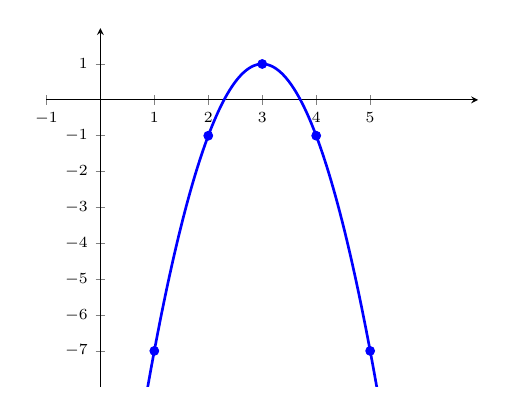
\begin{tikzpicture}[scale=0.8]
\begin{axis}[
xmin = -1, xmax = 7,
ymin = -8, ymax = 2,
xtick = {-1,0,...,5},
ytick = {-7,-6,...,1}
]
\addplot[color=blue, very thick, samples=200, smooth, domain=0:6] {-2*(x-3)^2 + 1};
\addplot[color=blue, mark=*, only marks] coordinates {(1,-7) (2,-1) (3,1) (4,-1) (5,-7)};
\end{axis}
\end{tikzpicture}
\end{minipage}
\begin{minipage}{0.4\textwidth}
\begin{align*}
    x-3 &= \pm \sqrt{\frac{1}{2}} \\[6pt]
    \onslide<2->{x-3 &= \pm \frac{\sqrt{2}}{2}} \\[6pt]
    \onslide<3->{x &= 3 \pm \frac{\sqrt{2}}{2}}
\end{align*}
\onslide<4->{$\left(3 \pm \frac{\sqrt{2}}{2},0\right)$} \\[6pt]
\onslide<5->{$y$-intercept: $(0,-17)$}
\end{minipage}
\end{frame}

\section{Convert between standard and general form of quadratic functions}

\begin{frame}{Standard and General Form of Quadratic Functions}
If $f$ is a quadratic function: \newline\\  
\begin{itemize}
    \item<+-> The \alert{general form} is $f(x) = ax^2+bx+c$
    \begin{itemize}
        \item<+-> $a$, $b$, and $c$ are real numbers
        \item<+-> $a \neq 0$    
    \end{itemize}   \vspace{8pt}
    \item<+-> The \alert{standard form} is $f(x) = a(x-h)^2 + k$
    \begin{itemize}
        \item<+-> Vertex is $(h,k)$
        \item<+-> $a \neq 0$
        \item<+-> $a$, $h$, and $k$ are real numbers
    \end{itemize}
\end{itemize}
\end{frame}

\begin{frame}{Converting From General to Standard Form}
    To convert from general form $f(x) = ax^2 + bx + c$ to standard form $f(x) = a(x-h)^2+k$ \newline\\
    \begin{enumerate}
        \onslide<2->{\item Find the vertex:}  \\[8pt]
        \begin{itemize}
            \onslide<2->{\item $x$-coordinate: $\frac{-b}{2a}$} \\[8pt]
            \onslide<2->{\item $y$-coordinate: Evaluate function at $x$-coordinate} \\[8pt]
            \onslide<2->{\item Or use graphing technology} \\[8pt]
        \end{itemize}
        \onslide<2->{\item Use the same value of $a$}
    \end{enumerate}
\end{frame}

\begin{frame}{Example 2}
Convert each to standard form.  \newline\\
(a) \quad $f(x) = x^2 - 4x + 3$ \newline\\
\onslide<2->{Vertex:} \newline\\
\onslide<3->{$x = \frac{-(-4)}{2(1)}$} \newline\\
\onslide<4->{$x = 2$} \newline\\
\onslide<5->{$y = 2^2 - 4(2) + 3$} \newline\\
\onslide<6->{$y = -1$}
\end{frame}

\begin{frame}{Example 2}
(a) \quad $f(x) = x^2 - 4x + 3$ \newline\\
Vertex: $(2,-1)$    \newline\\
\onslide<2->{$a = 1$}
\onslide<3->{\[f(x) = (x-2)^2 - 1\]}
\end{frame}

\begin{frame}{Example 2}
Convert each to standard form.  \newline\\
(b) \quad $g(x) = 6-x-x^2$  
\onslide<2->{\[g(x) = -x^2 - x + 6\]}
\begin{minipage}{0.55\textwidth}
\onslide<3->{
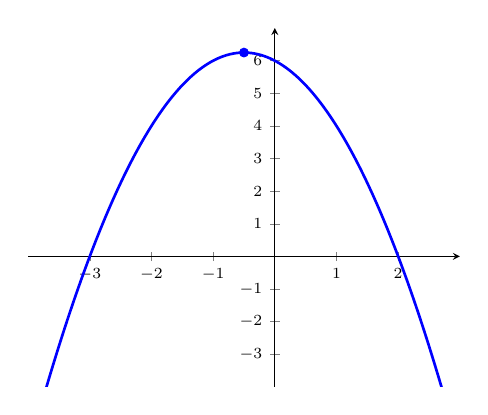
\begin{tikzpicture}[scale=0.8]
\begin{axis}[
xmin = -4, xmax = 3,
ymin = -4, ymax = 7,
xtick = {-3,-2,...,2},
ytick = {-3,-2,...,6}
]
\addplot[color=blue, very thick, samples=200, smooth] {-x^2-x+6};
\addplot[color=blue, mark=*] coordinates {(-0.5,6.25)};
\end{axis}
\end{tikzpicture}}
\end{minipage}
\begin{minipage}{0.4\textwidth}
\onslide<4->{Vertex: $\left(-\frac{1}{2},\frac{25}{4}\right)$} \\[12pt]
\onslide<5->{$a = -1$} \\[12pt]
\onslide<6->{$g(x) = -\left(x+\frac{1}{2}\right)^2 + \frac{25}{4}$}
\end{minipage}
\end{frame}

\begin{frame}{Axis of Symmetry}
The graphs of the parabolas have a line of symmetry called the \alert{axis of symmetry} that is a vertical line through the $x$-coordinate of the vertex:   \newline\\
\begin{minipage}{0.7\textwidth}
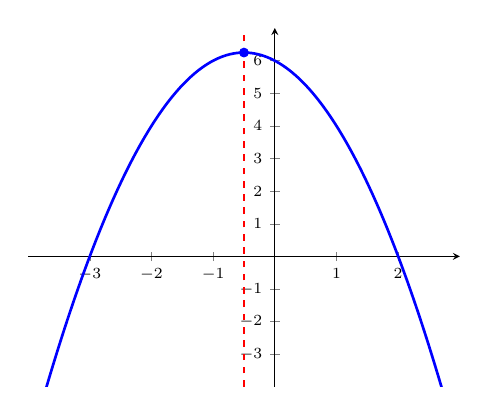
\begin{tikzpicture}[scale=0.8]
\begin{axis}[
xmin = -4, xmax = 3,
ymin = -4, ymax = 7,
xtick = {-3,-2,...,2},
ytick = {-3,-2,...,6}
]
\addplot[color=blue, very thick, samples=200, smooth] {-x^2-x+6};
\addplot[color=blue, mark=*] coordinates {(-0.5,6.25)};
\draw[dashed, very thick, red] (axis cs:-0.5,-4) -- (-0.5,7);
\end{axis}
\end{tikzpicture}
\end{minipage}
\begin{minipage}{0.2\textwidth}
\onslide<2->{\color{red}$x = -\frac{1}{2}$}
\end{minipage}
\end{frame}

\begin{frame}{Converting From Standard to General Form}
To convert from 
\[ f(x) = a(x-h)^2 + k \]
form to 
\[ f(x) = ax^2 + bx + c\]
form, just \textbf{do the math}.
\end{frame}

\begin{frame}{Example 3}
Convert $g(x) = (x+2)^2 - 3$ to general form.
\begin{align*}
    \onslide<2->{(x+2)^2 - 3 &= x^2 + 4x + 4 - 3} \\[8pt]
    \onslide<3->{&= x^2 + 4x + 1}
\end{align*}
\end{frame}

\end{document}
